\documentclass[11pt,a4paper]{article}

\usepackage[margin=1in]{geometry}
\usepackage{titlesec}
\usepackage{enumitem}
\usepackage{hyperref}
\usepackage{parskip}
\usepackage{graphicx}
\usepackage{float}
\usepackage{booktabs}
\usepackage{amsmath}

\hypersetup{colorlinks=true, linkcolor=blue, urlcolor=blue}

\titleformat{\section}{\large\bfseries}{\thesection}{0.5em}{}
\titleformat{\subsection}{\normalsize\bfseries}{\thesubsection}{0.5em}{}
\setlist{leftmargin=1.4em, topsep=2pt, itemsep=2pt}

\title{\vspace{-1.5cm}\textbf{PKCERT AI \& Software Development Internship \\ Task 07: Machine Learning Foundations}}
\author{Abdullah Amir}
\date{AI and Software Development \\ 10 July 2026}

\begin{document}

\maketitle
\vspace{-0.8cm}

This report covers the theory and the results. The full code, outputs, and plots
live in the notebook \texttt{ml\_foundations.ipynb}. The dataset is
\textbf{Auto MPG}: 398 cars, where the goal is to predict fuel economy
(\texttt{mpg}) from specs like weight, horsepower, and engine size.

% ----------------------------------------------------------------
\section*{Part A: Train/Test Split}

\textbf{Why we split.} A model that is scored on the same rows it trained on can
look great just by memorising them, and then fail on anything new. To get an
honest read on how it generalises, we fit the model on a \textbf{training set}
and measure it on a separate \textbf{test set} that the model never saw during
training. The gap between training and test performance is what tells us whether
the model actually learned the pattern or just the noise.

\textbf{Common ratios.} The right split depends on how much data there is.
\begin{itemize}
    \item \textbf{80/20} is the standard default and works well for most
    medium-sized datasets.
    \item \textbf{70/30} hands more rows to the test set, which gives a steadier
    performance estimate when the dataset is on the smaller side.
    \item \textbf{90/10} is fine for very large datasets, where even 10 percent is
    still tens of thousands of rows.
\end{itemize}

\textbf{The random\_state parameter.} \texttt{train\_test\_split} shuffles the
rows before cutting them, so without a fixed seed you get a different split every
run and slightly different scores each time. Setting \texttt{random\_state} to a
fixed number makes that shuffle deterministic, so the same rows land in the same
set on every run. That is what makes an experiment reproducible and makes two
models a fair comparison, since they are then tested on identical data.

\textbf{Validation set vs test set.} A validation set is a third slice carved out
of the training data and used \emph{during} development to tune settings and
choose between models. The test set is different: it is locked away and used only
once, at the very end, for a final unbiased score. Keeping them separate stops
choices made while tuning from leaking into the final number and flattering it.

% ----------------------------------------------------------------
\section*{Part B: Overfitting, Underfitting \& the Bias-Variance Tradeoff}

\textbf{Underfitting} happens when the model is too simple to capture the real
pattern, so it does poorly on both the training and the test data. Fitting a
straight line to data that clearly curves is the standard example: no matter how
you position the line, it cannot bend to follow the trend.

\textbf{Overfitting} is the opposite. The model is so flexible that it memorises
the noise in the training data along with the signal. It scores almost perfectly
on training data but poorly on the test set. A very high-degree polynomial that
wiggles through every single training point is the classic case, and we see
exactly this at degree 3 in the bonus section below.

\textbf{The tradeoff.} These two failures are the two ends of the same dial.
\emph{Bias} is error from wrong assumptions, a model too simple for the job, and
it drives underfitting. \emph{Variance} is error from being too sensitive to the
particular training rows, and it drives overfitting. As model complexity goes up,
bias falls but variance rises. Total error is the sum of the two, so the best
model sits at the balance point in the middle where that sum is lowest, not at
either extreme.

\textbf{Techniques to reduce overfitting.}
\begin{itemize}
    \item \textbf{Use a simpler model or fewer features} so there is less room to
    fit noise.
    \item \textbf{Regularization} (Ridge or Lasso) adds a penalty on large
    coefficients, which pulls the model back toward simplicity.
    \item \textbf{Cross-validation} tests on several splits so overfitting is
    caught early rather than hidden by one lucky split.
    \item \textbf{More training data} gives the model more real signal to learn
    from and less chance to memorise.
\end{itemize}

\textbf{How to diagnose it.} Compare the two scores. A high training score with a
much lower test score means overfitting (high variance). Low scores on both means
underfitting (high bias). Scores that are close together and both high means the
model generalises well. The plot below makes this visible: it trains polynomial
models of rising degree and tracks training against test error.

\begin{figure}[H]
    \centering
    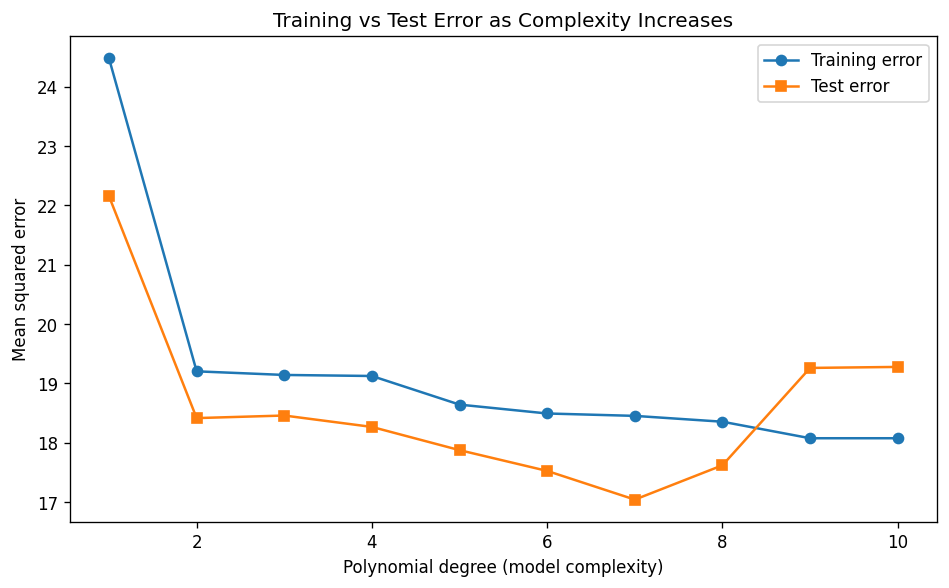
\includegraphics[width=0.70\textwidth]{figures/01_complexity_curve.png}
    \caption{At low degree both errors are high (underfitting). Past the sweet
    spot the test error climbs while training error keeps falling, which is
    overfitting.}
\end{figure}

% ----------------------------------------------------------------
\section*{Part C: Linear Regression Theory \& Implementation}

\textbf{The model.} Simple linear regression fits a straight line through the
data:
\[ y = mx + b \]
where $m$ is the slope (how much $y$ moves per unit of $x$) and $b$ is the
intercept (the value of $y$ when $x$ is zero). Multiple linear regression extends
this to several features at once, giving each its own weight:
\[ y = b + w_1 x_1 + w_2 x_2 + \dots + w_n x_n \]

\textbf{How the coefficients are learned.} The model chooses the weights that make
its predictions as close as possible to the real values. ``Close'' is measured by
a cost function, the Mean Squared Error:
\[ J = \frac{1}{N} \sum_{i=1}^{N} (y_i - \hat{y}_i)^2 \]
Minimising $J$ can be done two ways. The \textbf{normal equation}
$(X^T X)^{-1} X^T y$ solves for the best weights directly in one step, and this is
what scikit-learn's \texttt{LinearRegression} uses under the hood. Alternatively,
\textbf{gradient descent} starts from random weights and repeatedly nudges them in
the direction that lowers $J$ the fastest, taking small steps downhill until it
settles at the minimum. The normal equation is neat for a modest number of
features; gradient descent scales better to very large problems.

\textbf{Implementation.} Predicting \texttt{mpg} from \texttt{weight} alone learns
the line
\[ \text{mpg} = -0.0078 \times \text{weight} + 46.78, \qquad R^2 = 0.723 \]
The negative slope matches intuition: heavier cars use more fuel, so their
\texttt{mpg} is lower. Using all of the features together lifts $R^2$ to
\textbf{0.845} with an MSE of 8.34, a clear improvement over the single-feature
model.

\begin{figure}[H]
    \centering
    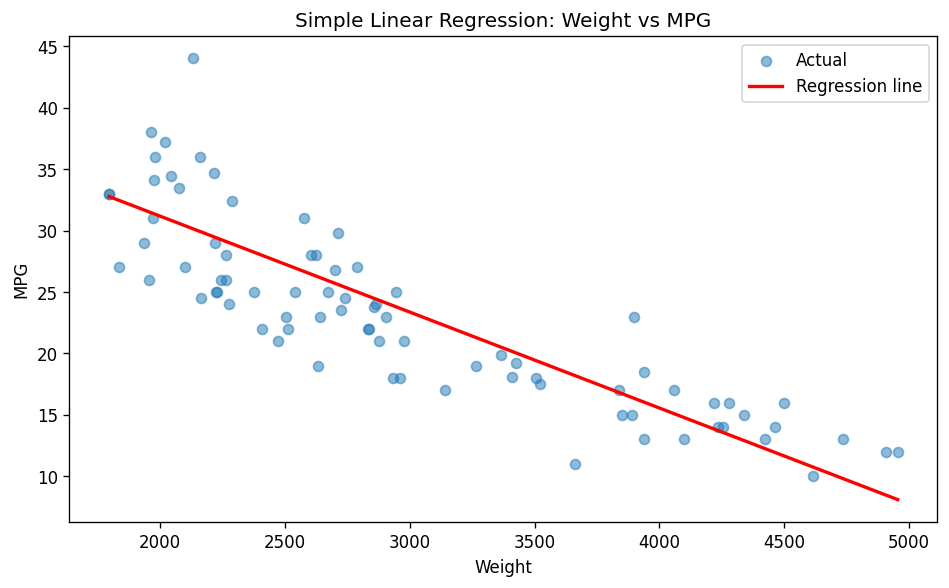
\includegraphics[width=0.60\textwidth]{figures/02_regression_line.png}
    \hfill
    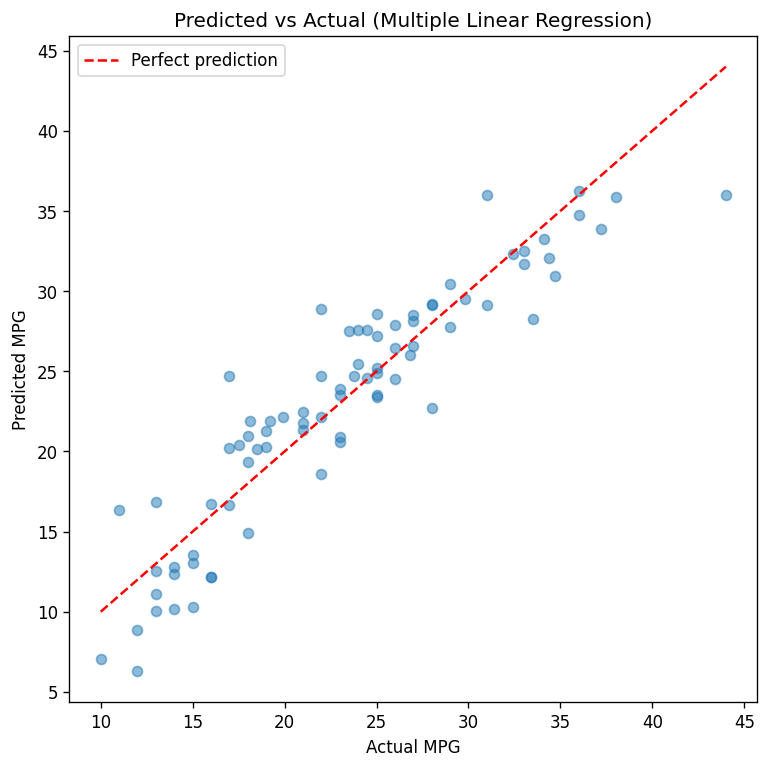
\includegraphics[width=0.36\textwidth]{figures/03_predicted_vs_actual.png}
    \caption{Left: the fitted line for weight vs MPG. Right: predicted vs actual
    MPG for the full model, with points hugging the diagonal.}
\end{figure}

% ----------------------------------------------------------------
\section*{Part D: Practical Results}

The raw CSV was cleaned by filling the 6 missing \texttt{horsepower} values with
the median, dropping the free-text \texttt{name} column, and one-hot encoding the
categorical \texttt{origin} column. The workflow was then refactored into four
reusable functions: \texttt{load\_data}, \texttt{split\_data},
\texttt{train\_model}, and \texttt{evaluate\_model}.

Training the same model on three split ratios shows the metrics barely move, so
the model is stable and not at the mercy of one particular split. Five-fold
cross-validation, which averages over five different folds, confirms it.

\begin{table}[H]
\centering
\begin{tabular}{lrr}
\toprule
\textbf{Split} & \textbf{MSE} & \textbf{$R^2$} \\
\midrule
60/40 & 9.85 & 0.828 \\
80/20 & 8.34 & 0.845 \\
90/10 & 10.65 & 0.826 \\
\midrule
5-fold CV & n/a & 0.814 (std 0.023) \\
\bottomrule
\end{tabular}
\caption{Stable metrics across ratios, backed up by cross-validation.}
\end{table}

The learning curve plots the training and cross-validation scores as the training
set grows. The two lines start far apart (the model does well on a tiny training
set but generalises poorly) and then converge to about $R^2 = 0.81$ as more data
is added. That small final gap is the sign of a healthy fit: no overfitting, since
the gap closed, and no underfitting, since the score settled high.

\begin{figure}[H]
    \centering
    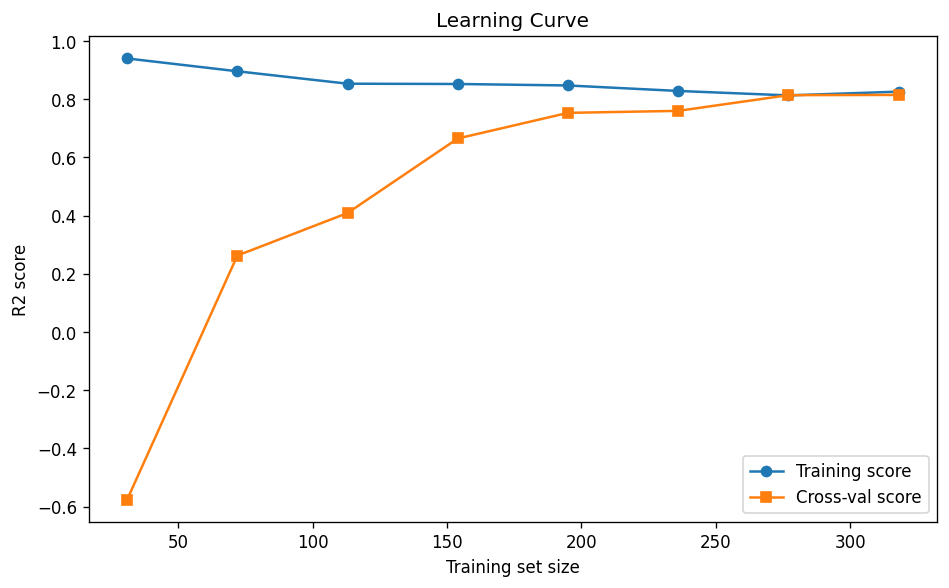
\includegraphics[width=0.66\textwidth]{figures/04_learning_curve.png}
    \caption{Training and cross-validation scores converging as data grows.}
\end{figure}

% ----------------------------------------------------------------
\section*{Bonus: Polynomial Regression}

Adding polynomial features lets the model fit curved relationships. Comparing
degrees 1 through 3 shows both the upside and the danger.

\begin{table}[H]
\centering
\begin{tabular}{lrr}
\toprule
\textbf{Degree} & \textbf{Train $R^2$} & \textbf{Test $R^2$} \\
\midrule
1 (plain linear) & 0.819 & 0.845 \\
2 & 0.899 & 0.895 \\
3 & 0.954 & 0.076 \\
\bottomrule
\end{tabular}
\caption{Degree 2 generalises best; degree 3 overfits badly.}
\end{table}

Degree 2 lifts both the training and the test score, so the extra curvature is
genuine signal and the model \textbf{generalises better}. Degree 3 tells the
opposite story: training $R^2$ climbs to 0.95 while test $R^2$ collapses to about
0.08. The model now has enough freedom to chase noise in the training data, which
is textbook \textbf{overfitting}. The takeaway is that more complexity is only
worth it while the test score keeps improving alongside the training score.

\vspace{0.4cm}
The notebook and README are on GitHub:
\url{https://github.com/AbdullahAmir06/ai-internship-abdullahamir}.

\end{document}
